\hypertarget{ux5f3aux5316ux5b66ux4e60ux7684ux57faux672cux77e5ux8bc6}{%
\chapter{强化学习的基本知识}\label{ux5f3aux5316ux5b66ux4e60ux7684ux57faux672cux77e5ux8bc6}}

\hypertarget{ux591aux81c2ux8001ux864eux673aux4e0eux4e0aux7f6eux4fe1ux754cucbux7b97ux6cd5}{%
\section{多臂老虎机与上置信界（UCB）算法}\label{ux591aux81c2ux8001ux864eux673aux4e0eux4e0aux7f6eux4fe1ux754cucbux7b97ux6cd5}}

\hypertarget{ux4e00ux591aux81c2ux8001ux864eux673amulti-armed-banditmab}{%
\subsection{一、多臂老虎机（multi-armed bandit，MAB）}\label{ux4e00ux591aux81c2ux8001ux864eux673amulti-armed-banditmab}}

在多臂老虎机问题（见图 2-1）中，有一个拥有~K根拉杆的老虎机，拉动每一根拉杆都对应一个关于奖励的概率分布R。我们每次拉动其中一根拉杆，就可以从该拉杆对应的奖励概率分布中获得一个奖励r。我们在各根拉杆的奖励概率分布未知的情况下，从头开始尝试，目标是在操作T~次拉杆后获得尽可能高的累积奖励。由于奖励的概率分布是未知的，因此我们需要在``探索拉杆的获奖概率''（探索）和``根据经验选择获奖最多的拉杆''（利用）中进行权衡。``采用怎样的操作策略才能使获得的累积奖励最高''便是多臂老虎机问题。

形式化表述：

多臂老虎机问题可以表示为一个元组 \((\mathcal{A}, \mathcal{R})\)，其中：

\begin{itemize}
\tightlist
\item
  \(\mathcal{A}\) 为动作集合，其中一个动作表示拉动一个拉杆。若多臂老虎机一共有 \(K\) 根拉杆，那么动作空间就是集合 \(\{a_1,\ldots,a_K\}\)，我们用 \(a_t \in \mathcal{A}\) 表示任意一个动作。
\item
  \(\mathcal{R}\) 为奖励概率分布，拉动每一根拉杆的动作 \(a\) 都对应一个奖励概率分布 \(R(r\mid a)\)，不同拉杆的奖励分布通常是不同的。
\end{itemize}

假设每个时间步只能拉动一个拉杆，多臂老虎机的目标为最大化一段时间步 \(T\) 内累积的奖励：

\[
\max \sum_{t=1}^{T} r_t,\qquad r_t \sim R(\cdot\mid a_t).
\]

其中 \(a_t\) 表示在第 \(t\) 时间步拉动某一拉杆的动作，\(r_t\) 表示动作 \(a_t\) 获得的奖励。

对于每一个动作 \(a\)，我们定义其期望奖励为

\[
Q(a)=\mathbb{E}_{r\sim R(\cdot\mid a)}[r].
\]

于是，至少存在一根拉杆，它的期望奖励不小于拉动其他任意一根拉杆，我们将该最优期望奖励表示为

\[
Q^{*}=\max_{a\in\mathcal{A}} Q(a).
\]

为了更加直观地观察某一拉杆的期望奖励与最优拉杆期望奖励之间的差距，我们引入``遗憾''（regret）概念。遗憾定义为当前动作与最优动作期望奖励之差，即

\[
R(a)=Q^{*}-Q(a).
\]

累积遗憾（cumulative regret）即操作 \(T\) 次拉杆后累积的遗憾总量。对于一次完整的 \(T\) 步决策 \(\{a_1,a_2,\ldots,a_T\}\)，累积遗憾为

\[
\mathcal{R}_T=\sum_{t=1}^{T} R(a_t).
\]

MAB 问题的目标是最大化累积奖励，等价于最小化累积遗憾。

为了知道拉动哪一根拉杆能获得更高的奖励，我们需要估计这根拉杆的期望奖励。由于只拉动一次拉杆获得的奖励存在随机性，所以需要多次拉动同一根拉杆，然后计算得到的多次奖励的期望。一个增量式估计流程如下：

\begin{enumerate}
\def\labelenumi{\arabic{enumi}.}
\tightlist
\item
  对于任意 \(a\in\mathcal{A}\)，初始化计数器 \(N(a)=0\) 和期望奖励估计值 \(\hat{Q}(a)=0\)。
\item
  对 \(t=1,\ldots,T\) 循环：

  \begin{itemize}
  \tightlist
  \item
    选取某根拉杆，该动作记为 \(a_t\)。
  \item
    得到奖励 \(r_t\)。
  \item
    更新计数器：\(N(a_t)=N(a_t)+1\)。
  \item
    更新期望奖励估计值：\(\hat{Q}(a_t)\leftarrow \hat{Q}(a_t)+\frac{1}{N(a_t)}[r_t-\hat{Q}(a_t)]\)。
  \end{itemize}
\end{enumerate}

注：如果将所有数求和再除以次数，其缺点是每次更新的时间复杂度和空间复杂度均为 \(O(n)\)。而采用增量式更新，时间复杂度和空间复杂度均为 \(O(1)\)。

一个最简单的策略就是一直采取第一个动作，但这就非常依赖运气的好坏。如果运气绝佳，可能拉动的刚好是能获得最大期望奖励的拉杆，即最优拉杆；但如果运气很糟糕，获得的就有可能是最小的期望奖励。

在多臂老虎机问题中，一个经典的问题就是探索与利用的平衡问题。探索（exploration）是指尝试拉动更多可能的拉杆，这根拉杆不一定会获得最大的奖励，但这种方案能够摸清楚所有拉杆的获奖情况。例如，对于一个 10 臂老虎机，我们要把所有的拉杆都拉动一下才知道哪根拉杆可能获得最大的奖励。利用（exploitation）是指拉动已知期望奖励最大的那根拉杆，由于已知的信息仅仅来自有限次的交互观测，所以当前的最优拉杆不一定是全局最优的。例如，对于一个 10 臂老虎机，我们只拉动过其中 3 根拉杆，接下来就一直拉动这 3 根拉杆中期望奖励最大的那根拉杆，但很有可能期望奖励最大的拉杆在剩下的 7 根当中，即使我们对 10 根拉杆各自都尝试了 20 次，发现 5 号拉杆的经验期望奖励是最高的，但仍然存在着微小的概率---另一根 6 号拉杆的真实期望奖励是比 5 号拉杆更高的。

于是在多臂老虎机问题中，设计策略时就需要平衡探索和利用的次数，使得累积奖励最大化。一个比较常用的思路是在开始时做比较多的探索，在对每根拉杆都有比较准确的估计后，再进行利用。目前已有一些比较经典的算法来解决这个问题，例如epsilon-贪婪算法、上置信界算法和汤普森采样算法等。

\hypertarget{ux4e8cepsilon-ux8d2aux5a6aux7b97ux6cd5}{%
\subsection{二、epsilon-贪婪算法}\label{ux4e8cepsilon-ux8d2aux5a6aux7b97ux6cd5}}

完全贪婪算法即在每一时刻采取期望奖励值最大的动作（拉动拉杆），这就是纯粹的利用，而没有探索。所以我们通常需要对完全贪婪算法进行一些修改，其中比较经典的一种方法为 \(\epsilon\)-贪婪（\(\epsilon\)-Greedy）算法。

\(\epsilon\)-贪婪算法在完全贪婪算法的基础上添加了噪声，每次以概率 \(1-\epsilon\) 选择以往经验中期望奖励值最大的那根拉杆（利用），以概率 \(\epsilon\) 随机选择一根拉杆（探索），公式如下：

\[
a_t=
\begin{cases}
\arg\max\limits_{a\in\mathcal{A}} \hat{Q}(a), & \mathcjk{采样概率 } 1-\epsilon,\\
\mathcjk{从 }\mathcal{A}\mathcjk{ \mathcjk{中随机选择}}, & \mathcjk{采样概率 } \epsilon.
\end{cases}
\]

\hypertarget{ux4e09ux4e0aux7f6eux4fe1ux754cucbux7b97ux6cd5}{%
\subsubsection{（三）上置信界（UCB）算法}\label{ux4e09ux4e0aux7f6eux4fe1ux754cucbux7b97ux6cd5}}

设想这样一种情况：对于一台双臂老虎机，其中第一根拉杆只被拉动过一次；第二根拉杆被拉动过很多次，我们对它的奖励分布已经有了大致的把握。这时你会怎么做？或许你会进一步尝试拉动第一根拉杆，从而更加确定其奖励分布。这种思路主要是基于不确定性，因为此时第一根拉杆只被拉动过一次，它的不确定性很高。一根拉杆的不确定性越大，它就越具有探索的价值，因为探索之后我们可能发现它的期望奖励很大。我们在此引入不确定性度量U(a)，它会随着一个动作被尝试次数的增加而减小。我们可以使用一种基于不确定性的策略来综合考虑现有的期望奖励估值和不确定性，其核心问题是如何估计不确定性。

上置信界（upper confidence bound, UCB）算法是一种经典的基于不确定性的策略算法，它的思想用到了一个非常著名的数学原理：霍夫丁不等式（Hoeffding's inequality）。在霍夫丁不等式中，令 \(X_1,\ldots,X_n\) 为 \(n\) 个独立同分布的随机变量，取值范围为 \([0,1]\)，其经验期望为

\[
\bar{x}_n=\frac{1}{n}\sum_{j=1}^{n} X_j,
\]

则有

\[
\Pr\{\mathbb{E}[X]\ge \bar{x}_n+u\}\le e^{-2nu^{2}}.
\]

现在我们将霍夫丁不等式运用于多臂老虎机问题中。将 \(\hat{Q}_t(a)\) 代入 \(\bar{x}_n\)，不等式中的参数 \(u=\hat{U}_t(a)\) 代表不确定性度量。给定一个概率

\[
p=e^{-2N_t(a)\hat{U}_t(a)^{2}},
\]

根据上述不等式，\(Q_t(a)<\hat{Q}_t(a)+\hat{U}_t(a)\) 至少以概率 \(1-p\) 成立。当 \(p\) 很小时，\(Q_t(a)<\hat{Q}_t(a)+\hat{U}_t(a)\) 就会在很大概率上成立，\(\hat{Q}_t(a)+\hat{U}_t(a)\) 便是期望奖励上界。

此时，上置信界算法便选取期望奖励上界最大的动作：

\[
a_t=\arg\max_{a\in\mathcal{A}}[\hat{Q}_t(a)+\hat{U}_t(a)].
\]

所谓的``误判''（或者说我们在设定 \(p\) 时想要规避的那个``小概率事件''），指的正是：拉杆的真实期望值竟然比``我们观察到的平均值加上不确定性红利''还要高。用数学公式表示，就是当下面这个事件发生时，我们视为``误判''：

\[
Q(a)>\hat{Q}_t(a)+\hat{U}_t(a).
\]

如果我们希望降低``把一个很好的杆误认为不好，错过好的解''的概率 \(p\)，我们就要选择把 \(u\) 放宽，拉高上置信界，从而鼓励更多的探索。

当设定p后，我们可以得出不确定度u的值：

\[
u=\sqrt{\frac{-\ln p}{2n}}.
\]

我们一般设置 \(p=1/t\)。在 \(t\) 较小的时候，鼓励算法先通过少数探索快速找到一个近似最优；在 \(t\) 较大的时候，如果一个臂很久没有被选中（\(n\) 没变），但总时间 \(t\) 增加了，那么它的探索加分项就会变大。这会强行把它的得分拉高，让算法去``再试一次''这个臂，以满足我们随时间日益严苛的置信度要求。否则，臂只要被选中一次，\(u\) 就会减小一点，尽管``冷门臂''的 \(u\) 始终更大，但随着时间推移和 \(n\) 的增大，所有臂的 \(u\) 都会逐渐接近 \(0\)，使得这一项远远小于 \(Q\)，最终不起作用，可能让算法收敛向一个次优解。

这里还可以进一步写成经典的 UCB 形式：

\[
a_t=\arg\max_{a\in\mathcal{A}}[\hat{Q}_t(a)+\sqrt{\frac{2\ln t}{N_t(a)}}].
\]

技术彩蛋：在更严谨的 UCB1 推导中，常取 \(p=t^{-4}\)，由此得到探索项 \(\sqrt{\frac{2\ln t}{N_t(a)}}\)。如果只取 \(p=1/t\)，则 \(\sum_t 1/t\) 发散；而 \(p=t^{-4}\) 对应的级数收敛，更便于从数学上证明遗憾上界。但无论取 \(1/t\) 还是 \(t^{-4}\)，核心都是利用 \(\ln t\) 维持长期探索动力。

\hypertarget{ux56dbux6c64ux666eux68eeux91c7ux6837}{%
\subsection{四、汤普森采样}\label{ux56dbux6c64ux666eux68eeux91c7ux6837}}

\begin{enumerate}
\def\labelenumi{\arabic{enumi}.}
\tightlist
\item
  核心思想
\end{enumerate}

如果说 UCB 是一个严谨的数学家（计算严格的边界，绝不冒险漏掉任何可能性），那么汤普森采样就是一个智慧的赌徒（基于概率分布模拟未来，用随机性来对抗未知）。UCB 是频率学派的方法：它根据观察到的数据计算一个固定的数值（平均值 + 误差项）。汤普森采样则是贝叶斯学派的方法。它的核心逻辑是：我不直接估计拉杆的中奖率是多少，而是维护一个``中奖率的概率分布''。在每一步，我从每根拉杆的分布里随机抽一个数（Sample），假装这个数就是这根拉杆的真实能力，然后选那个抽出来数值最大的拉杆。

对于陌生的拉杆：我不知道它中奖率是多少，所以我认为它可能是0到1之间的任何值（分布很宽，很平）。

对于熟悉的拉杆：我知道它中奖率大概是 80\%，所以我认为它的概率分布主要集中在 0.75 到 0.85 之间（分布很窄，很尖）。

\begin{enumerate}
\def\labelenumi{\arabic{enumi}.}
\setcounter{enumi}{1}
\tightlist
\item
  数学模型：Beta分布
\end{enumerate}

在处理二元奖励（赢/输，\(1/0\)）的老虎机问题时，汤普森采样通常使用 Beta 分布（Beta Distribution）作为共轭先验。

不需要被名字吓到，你只需要记住 Beta 分布有两个参数：\(\alpha\) 和 \(\beta\)。

\[
f(x;\alpha,\beta)=\mathrm{Beta}(\alpha,\beta)
\]

在老虎机场景下，它们的物理含义极其简单：

\begin{itemize}
\tightlist
\item
  \(\alpha\)（Alpha）：代表该拉杆``赢（获得奖励 1）''的次数 \(+1\)。
\item
  \(\beta\)（Beta）：代表该拉杆``输（获得奖励 0）''的次数 \(+1\)。
\end{itemize}

为什么这么做？

Beta 分布的形状决定了我们对拉杆的看法：

\begin{enumerate}
\def\labelenumi{\arabic{enumi}.}
\item
  初始状态（\(\alpha=1,\beta=1\)）：相当于均匀分布。我觉得中奖率在 \([0,1]\) 之间任意一个值的概率都一样。这就是``无知''。
\item
  赢多输少（\(\alpha=100,\beta=10\)）：曲线会在 \(0.9\) 附近高高隆起。这意味着``我很确定它是个好拉杆''。
\item
  尝试极少（\(\alpha=2,\beta=1\)）：曲线比较平缓。这意味着``它可能很好，也可能很差，不确定性很大''。
\item
  算法流程
\end{enumerate}

汤普森采样的步骤非常简洁，不需要像 UCB 那样计算复杂的根号和对数：

\begin{enumerate}
\def\labelenumi{\arabic{enumi}.}
\tightlist
\item
  初始化：给每根拉杆 \(k\) 设定两个计数器 \(\alpha_k=1,\beta_k=1\)。
\item
  循环每一步 \(t\)：

  \begin{itemize}
  \item
    采样（Sample）：对于每一根拉杆 \(k\)，从其对应的分布 \(\mathrm{Beta}(\alpha_k,\beta_k)\) 中随机抽取一个样本值 \(\theta_k\sim \mathrm{Beta}(\alpha_k,\beta_k)\)。
  \item
    选择（Select）：选择 \(\theta_k\) 最大的那根拉杆（记为动作 \(A_t\)）。
  \item
    观察（Observe）：拉动拉杆 \(A_t\)，得到奖励 \(r\)（\(0\) 或 \(1\)）。
  \item
    更新（Update）：更新参数（贝叶斯推断）：

    \begin{itemize}
    \tightlist
    \item
      如果赢了（\(r=1\)）：\(\alpha_{A_t}\leftarrow \alpha_{A_t}+1\)
    \item
      如果输了（\(r=0\)）：\(\beta_{A_t}\leftarrow \beta_{A_t}+1\)
    \end{itemize}
  \end{itemize}
\end{enumerate}

\hypertarget{ux53c2ux8003ux6587ux732e-40}{%
\subsection{参考文献}\label{ux53c2ux8003ux6587ux732e-40}}

\begin{itemize}
\tightlist
\item
  \href{https://hrl.boyuai.com/}{《动手学强化学习》}.
\item
  Auer, P., Cesa-Bianchi, N., \& Fischer, P. (2002). \href{https://link.springer.com/article/10.1023/A:1013689704352}{Finite-time Analysis of the Multiarmed Bandit Problem}. Machine Learning.
\end{itemize}

\clearpage

\hypertarget{ux9a6cux5c14ux53efux592bux8fc7ux7a0b}{%
\section{马尔可夫过程}\label{ux9a6cux5c14ux53efux592bux8fc7ux7a0b}}

首先说明：强化学习是一种训练方法（和监督学习等相对应），而不是一种模型架构或优化算法。

\hypertarget{ux4e00ux9a6cux5c14ux53efux592bux8fc7ux7a0b}{%
\subsection{一、马尔可夫过程}\label{ux4e00ux9a6cux5c14ux53efux592bux8fc7ux7a0b}}

多臂老虎机中，智能体的行动并不对环境产生影响，但真实世界并非如此。我们引入马尔可夫过程的概念。

马尔可夫过程（Markov process）指具有马尔可夫性质的随机过程，也被称为马尔可夫链（Markov chain）。我们通常用元组 \((\mathcal{S},P)\) 描述一个马尔可夫过程，其中 \(\mathcal{S}\) 是有限数量的状态集合，\(P\) 是状态转移矩阵（state transition matrix）。假设一共有 \(n\) 个状态，此时 \(\mathcal{S}=\{s_1,s_2,\ldots,s_n\}\)，状态转移矩阵可以写成：

\[
P=
\begin{bmatrix}
P(s_1\mid s_1) & \cdots & P(s_n\mid s_1)\\
\vdots & \ddots & \vdots\\
P(s_1\mid s_n) & \cdots & P(s_n\mid s_n)
\end{bmatrix}.
\]

矩阵 \(P\) 中第 \(i\) 行第 \(j\) 列元素

\[
P(s_j\mid s_i)=P(S_{t+1}=s_j\mid S_t=s_i)
\]

表示从状态 \(s_i\) 转移到状态 \(s_j\) 的概率。对于任意状态 \(s_i\)，从它出发到达其他状态的概率和必须为 \(1\)，即状态转移矩阵的每一行之和为 \(1\)。

\begin{figure}[htbp]
\centering
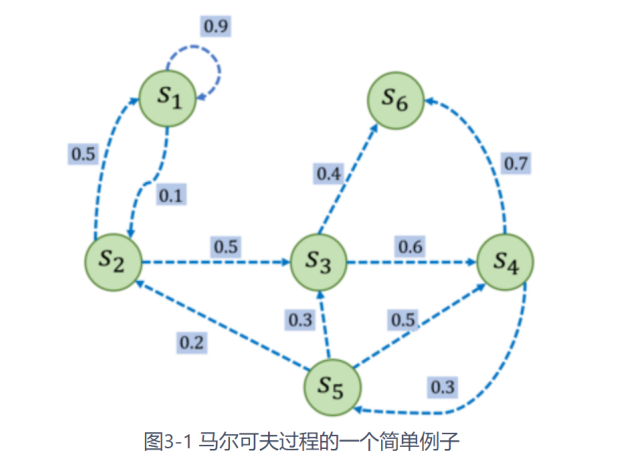
\includegraphics{images/image-0012.png}
\caption{马尔可夫过程状态转移示意图}
\end{figure}

给定一个马尔可夫过程，我们就可以从某个状态出发，根据它的状态转移矩阵生成一个状态序列（episode），这个步骤也被叫作采样（sampling）。例如，从 \(s_1\) 出发，可以生成序列 \(s_1\to s_2\to s_3\to s_6\)，或序列 \(s_1\to s_1\to s_2\to s_3\to s_4\to s_5\to s_3\to s_6\) 等。生成这些序列的概率和状态转移矩阵有关。

\hypertarget{ux4e8cux9a6cux5c14ux53efux592bux5956ux52b1ux8fc7ux7a0b}{%
\subsection{二、马尔可夫奖励过程}\label{ux4e8cux9a6cux5c14ux53efux592bux5956ux52b1ux8fc7ux7a0b}}

\hypertarget{ux56deux62a5}{%
\subsubsection{1. 回报}\label{ux56deux62a5}}

在马尔可夫过程的基础上加入奖励函数 \(r\) 和折扣因子 \(\gamma\)，就可以得到马尔可夫奖励过程（Markov reward process）。一个马尔可夫奖励过程由 \((\mathcal{S},P,r,\gamma)\) 构成，各个组成元素的含义如下：

\begin{itemize}
\tightlist
\item
  \(\mathcal{S}\) 是有限状态集合。
\item
  \(P\) 是状态转移矩阵。
\item
  \(r\) 是奖励函数，某个状态 \(s\) 的奖励 \(r(s)\) 指转移到该状态时可以获得奖励的期望。
\item
  \(\gamma\) 是折扣因子（discount factor），取值范围为 \([0,1)\)。引入折扣因子的原因是远期利益具有一定不确定性，有时我们更希望尽快获得一些奖励，所以会对远期利益进行折扣。\(\gamma\) 接近 \(1\) 时更关注长期累计奖励，接近 \(0\) 时更关注短期奖励。
\end{itemize}

在一个马尔可夫奖励过程中，从第 \(t\) 时刻状态 \(S_t\) 开始，直到终止状态时，所有奖励的衰减之和称为回报 \(G_t\)（return），公式如下：

\[
G_t=R_t+\gamma R_{t+1}+\gamma^{2} R_{t+2}+\cdots
=\sum_{k=0}^{\infty}\gamma^{k} R_{t+k}.
\]

以LLM为例：每次生成就是一次``状态转移''（已有全文即为状态），行动就是从词表（几万个词）中按概率选一个词（token），转移到下一个状态（新的全文）；奖励函数可以对某个状态（结果）或者某个过程进行奖励。

\hypertarget{ux4ef7ux503cux51fdux6570}{%
\subsubsection{2. 价值函数}\label{ux4ef7ux503cux51fdux6570}}

在马尔可夫奖励过程中，一个状态的期望回报（即从这个状态出发的未来累计奖励的期望）被称为这个状态的价值（value）。所有状态的价值组成了价值函数（value function），价值函数的输入为某个状态，输出为这个状态的价值。我们将价值函数写成

\[
V(s)=\mathbb{E}[G_t\mid S_t=s].
\]

进一步展开可得：

\[
\begin{aligned}
V(s)
&=\mathbb{E}[G_t\mid S_t=s]\\
&=\mathbb{E}[R_t+\gamma R_{t+1}+\gamma^{2} R_{t+2}+\cdots\mid S_t=s]\\
&=\mathbb{E}[R_t+\gamma(R_{t+1}+\gamma R_{t+2}+\cdots)\mid S_t=s]\\
&=\mathbb{E}[R_t+\gamma G_{t+1}\mid S_t=s]\\
&=\mathbb{E}[R_t+\gamma V(S_{t+1})\mid S_t=s].
\end{aligned}
\]

在上式的最后一个等号中，一方面，即时奖励的期望正是奖励函数的输出，即 \(\mathbb{E}[R_t\mid S_t=s]=r(s)\)；另一方面，等式中剩余部分 \(\mathbb{E}[\gamma V(S_{t+1})\mid S_t=s]\) 可以根据从状态 \(s\) 出发的转移概率得到，于是得到：

\[
V(s)=r(s)+\gamma\sum_{s'\in\mathcal{S}}P(s'\mid s)V(s').
\]

上式就是马尔可夫奖励过程中非常有名的贝尔曼方程（Bellman equation），对于每一个状态都成立。若一个马尔可夫奖励过程一共有 \(n\) 个状态，即 \(\mathcal{S}=\{s_1,s_2,\ldots,s_n\}\)，我们将所有状态的价值表示成一个列向量 \(\mathbf{V}=[V(s_1),V(s_2),\ldots,V(s_n)]^{\top}\)，同理，转移矩阵 \(P\) 可以写成矩阵形式，奖励函数写成列向量 \(\mathbf{R}=[r(s_1),r(s_2),\ldots,r(s_n)]^{\top}\)。于是贝尔曼方程可以写成：

\[
\mathbf{V}=\mathbf{R}+\gamma P\mathbf{V}.
\]

我们可以直接根据矩阵运算求解：

\[
\begin{aligned}
\mathbf{V}&=\mathbf{R}+\gamma P\mathbf{V},\\
(I-\gamma P)\mathbf{V}&=\mathbf{R},\\
\mathbf{V}&=(I-\gamma P)^{-1}\mathbf{R}.
\end{aligned}
\]

上述解析解的计算复杂度是 \(O(n^{3})\)，其中 \(n\) 是状态个数，因此这种方法只适用于很小的马尔可夫奖励过程。求解较大规模的马尔可夫奖励过程中的价值函数时，可以使用动态规划（dynamic programming）、蒙特卡洛方法（Monte-Carlo method）和时序差分（temporal difference）等方法。

\hypertarget{ux4e09ux9a6cux5c14ux53efux592bux51b3ux7b56ux8fc7ux7a0b}{%
\subsection{三、马尔可夫决策过程}\label{ux4e09ux9a6cux5c14ux53efux592bux51b3ux7b56ux8fc7ux7a0b}}

智能体的策略（policy）通常用字母 \(\pi\) 表示。策略

\[
\pi(a\mid s)=P(A_t=a\mid S_t=s)
\]

是一个函数，表示在输入状态 \(s\) 的情况下采取动作 \(a\) 的概率。当一个策略是确定性策略（deterministic policy）时，它在每个状态下只输出一个确定性的动作，即只有该动作的概率为 \(1\)，其他动作的概率为 \(0\)；当一个策略是随机性策略（stochastic policy）时，它在每个状态下输出的是关于动作的概率分布，然后根据该分布进行采样就可以得到一个动作。

在 MDP 中，由于马尔可夫性质的存在，策略只需要与当前状态有关，不需要考虑历史状态。回顾在 MRP 中的价值函数，在 MDP 中也同样可以定义类似的价值函数。但此时的价值函数与策略有关，这意味着对于两个不同的策略来说，它们在同一个状态下的价值也可能是不同的：不同策略会采取不同动作，从而之后会遇到不同状态并获得不同奖励，所以它们的累积奖励期望也就不同。

我们用 \(V^{\pi}(s)\) 表示在 MDP 中基于策略 \(\pi\) 的状态价值函数（state-value function），定义为从状态 \(s\) 出发遵循策略 \(\pi\) 能获得的期望回报：

\[
V^{\pi}(s)=\mathbb{E}_{\pi}[G_t\mid S_t=s].
\]

不同于 MRP，在 MDP 中由于动作的存在，我们还可以定义动作价值函数（action-value function）。我们用 \(Q^{\pi}(s,a)\) 表示在 MDP 遵循策略 \(\pi\) 时，对当前状态 \(s\) 执行动作 \(a\) 得到的期望回报：

\[
Q^{\pi}(s,a)=\mathbb{E}_{\pi}[G_t\mid S_t=s,A_t=a].
\]

状态价值函数和动作价值函数之间的关系为：在使用策略 \(\pi\) 时，状态 \(s\) 的价值等于在该状态下基于策略 \(\pi\) 采取所有动作的概率与相应动作价值相乘再求和的结果：

\[
V^{\pi}(s)=\sum_{a\in\mathcal{A}}\pi(a\mid s)Q^{\pi}(s,a).
\]

使用策略 \(\pi\) 时，状态 \(s\) 下采取动作 \(a\) 的价值等于即时奖励加上经过衰减后的所有可能下一状态的价值期望：

\[
Q^{\pi}(s,a)=r(s,a)+\gamma\sum_{s'\in\mathcal{S}}P(s'\mid s,a)V^{\pi}(s').
\]

\hypertarget{ux56dbux8d1dux5c14ux66fcux671fux671bux65b9ux7a0b}{%
\subsection{四、贝尔曼期望方程}\label{ux56dbux8d1dux5c14ux66fcux671fux671bux65b9ux7a0b}}

在贝尔曼方程中加上``期望''二字，是为了与接下来的贝尔曼最优方程进行区分。通过简单推导即可分别得到状态价值函数和动作价值函数的贝尔曼期望方程（Bellman expectation equation）：

\[
\begin{aligned}
V^{\pi}(s)
&=\mathbb{E}_{\pi}[R_t+\gamma V^{\pi}(S_{t+1})\mid S_t=s]\\
&=\sum_{a\in\mathcal{A}}\pi(a\mid s)
(r(s,a)+\gamma\sum_{s'\in\mathcal{S}}P(s'\mid s,a)V^{\pi}(s')),
\end{aligned}
\]

\[
\begin{aligned}
Q^{\pi}(s,a)
&=\mathbb{E}_{\pi}[R_t+\gamma Q^{\pi}(S_{t+1},A_{t+1})\mid S_t=s,A_t=a]\\
&=r(s,a)+\gamma\sum_{s'\in\mathcal{S}}P(s'\mid s,a)
\sum_{a'\in\mathcal{A}}\pi(a'\mid s')Q^{\pi}(s',a').
\end{aligned}
\]

\hypertarget{ux4e94ux8d1dux5c14ux66fcux6700ux4f18ux65b9ux7a0b}{%
\subsection{五、贝尔曼最优方程}\label{ux4e94ux8d1dux5c14ux66fcux6700ux4f18ux65b9ux7a0b}}

强化学习的目标通常是找到一个策略，使得智能体从初始状态出发能够获得最多的期望回报。我们首先定义策略之间的偏序关系：当且仅当对于任意状态 \(s\) 都有 \(V^{\pi}(s)\ge V^{\pi'}(s)\) 时，记 \(\pi\succ \pi'\)。于是在有限状态和动作集合的 MDP 中，至少存在一个策略比其他所有策略都好，或者至少存在一个策略不差于其他所有策略，这个策略就是最优策略（optimal policy）。最优策略可能有很多个，我们都将其表示为 \(\pi^{*}(s)\)。

最优策略都有相同的状态价值函数，我们称之为最优状态价值函数：

\[
V^{*}(s)=\max_{\pi}V^{\pi}(s),\qquad \forall s\in\mathcal{S}.
\]

同理，我们定义最优动作价值函数：

\[
Q^{*}(s,a)=\max_{\pi}Q^{\pi}(s,a),\qquad \forall s\in\mathcal{S},a\in\mathcal{A}.
\]

为了使 \(Q^{\pi}(s,a)\) 最大，我们需要在当前状态动作对 \((s,a)\) 之后都执行最优策略，于是得到了最优状态价值函数和最优动作价值函数之间的关系：

\[
Q^{*}(s,a)=r(s,a)+\gamma\sum_{s'\in\mathcal{S}}P(s'\mid s,a)V^{*}(s').
\]

这与普通策略下的状态价值函数和动作价值函数之间的关系一样。另一方面，最优状态价值是选择此时使最优动作价值最大的那个动作时的状态价值：

\[
V^{*}(s)=\max_{a\in\mathcal{A}}Q^{*}(s,a).
\]

根据 \(V^{*}(s)\) 和 \(Q^{*}(s,a)\) 的关系，我们可以得到贝尔曼最优方程（Bellman optimality equation）：

\[
V^{*}(s)=\max_{a\in\mathcal{A}}\bigl(r(s,a)+\gamma\sum_{s'\in\mathcal{S}}P(s'\mid s,a)V^{*}(s')\bigr).
\]

\[
Q^{*}(s,a)=r(s,a)+\gamma\sum_{s'\in\mathcal{S}}P(s'\mid s,a)
\max_{a'\in\mathcal{A}}Q^{*}(s',a').
\]

我们发现，和贝尔曼期望方程与策略 \(\pi\) 挂钩不同的是，贝尔曼最优方程与策略 \(\pi\) 无关，只与环境的状态转移特征有关。

\hypertarget{ux53c2ux8003ux6587ux732e-41}{%
\subsection{参考文献}\label{ux53c2ux8003ux6587ux732e-41}}

\begin{itemize}
\tightlist
\item
  \href{https://hrl.boyuai.com/}{《动手学强化学习》}.
\end{itemize}

\clearpage

\hypertarget{ux72b6ux6001ux5206ux5e03ux4e0eux5360ux7528ux5ea6ux91cf}{%
\section{状态分布与占用度量}\label{ux72b6ux6001ux5206ux5e03ux4e0eux5360ux7528ux5ea6ux91cf}}

\hypertarget{ux4e00ux72b6ux6001ux5206ux5e03ux548cux5360ux7528ux5ea6ux91cfux7684ux5b9aux4e49}{%
\subsection{一、状态分布和占用度量的定义}\label{ux4e00ux72b6ux6001ux5206ux5e03ux548cux5360ux7528ux5ea6ux91cfux7684ux5b9aux4e49}}

状态分布定义为智能体处于状态 \(s\) 的折扣后概率：

定义了 \(\nu^\pi(s)\)，即在策略 \(\pi\) 下的折扣状态访问分布：

\[
\nu^\pi(s) = (1-\gamma)\sum_{t=0}^{\infty}\gamma^t P_t^\pi(s)
\]

\(P_t^\pi(s)\)：表示在时刻 \(t\)，智能体处于状态 \(s\) 的概率。

\(\gamma\)：折扣因子（Discount Factor），\(0 \le \gamma < 1\)。

\(1-\gamma\)：归一化因子（Normalization Factor）。

进而可以定义占用度量，即智能体在s发出动作a的折扣后概率：

\[
\rho^\pi(s,a) = (1-\gamma)\sum_{t=0}^{\infty}\gamma^t P_t^\pi(s)\pi(a|s)
\]

此时有关系：

\[
\rho^\pi(s,a) = \nu^\pi(s)\pi(a|s)
\]

\hypertarget{ux4e8cux539fux7406ux63a8ux5bfc}{%
\subsection{二、原理推导}\label{ux4e8cux539fux7406ux63a8ux5bfc}}

\begin{enumerate}
\def\labelenumi{\arabic{enumi}.}
\tightlist
\item
  为什么需要折扣因子？
\end{enumerate}

我们通常希望最大化累积折扣回报：

\[
J(\pi) = \mathbb{E}_\pi\left[\sum_{t=0}^{\infty}\gamma^t R(s_t,a_t)\right]
\]

利用期望的线性性质，我们可以把求和号拿到期望外面：

\[
J(\pi) = \sum_{t=0}^{\infty}\gamma^t\mathbb{E}_\pi[R(s_t,a_t)]
\]

\[
J(\pi) = \sum_{t=0}^{\infty}\gamma^t\sum_{s,a}P_t^\pi(s)\pi(a|s)R(s,a)
\]

现在，我们将对于 \(s\) 和 \(a\) 的求和提到最前面：

\[
J(\pi) = \sum_{s,a}R(s,a)\left(\sum_{t=0}^{\infty}\gamma^t P_t^\pi(s)\pi(a|s)\right)
\]

括号中的这一项是未归一化的占用度量。为了让这一项变成概率分布（和为 1），我们乘以并除以 \((1-\gamma)\)：

\[
J(\pi) = \frac{1}{1-\gamma}\sum_{s,a}R(s,a)\left((1-\gamma)\sum_{t=0}^{\infty}\gamma^t P_t^\pi(s)\pi(a|s)\right)
\]

其中括号中的部分就是 \(\rho^\pi(s,a)\)，因此：

\[
J(\pi) = \frac{1}{1-\gamma}\sum_{s,a}\rho^\pi(s,a)R(s,a) = \frac{1}{1-\gamma}\mathbb{E}_{(s,a)\sim\rho^\pi}[R(s,a)]
\]

在强化学习中，我们的目标往往是找到一个好的策略。策略可以用概率分布表示，优化目标正是让回报 \(R\) 在 \(\rho^\pi\) 的概率分布下的数学期望最大化。这样一来，问题就转化为寻找这样的概率分布；状态-动作对在分布中的概率，等于该状态-动作对对总价值的贡献权重，符合我们对马尔可夫决策过程的认知。

\begin{enumerate}
\def\labelenumi{\arabic{enumi}.}
\setcounter{enumi}{1}
\tightlist
\item
  为什么需要归一化因子？
\end{enumerate}

这是一个非常关键的数学细节。我们需要证明 \(\nu^\pi(s)\) 是一个合法的概率分布，即其对所有状态求和必须为 1。

推导如下：我们对所有状态 \(s\) 求和：

\[
\sum_s \nu^\pi(s) = \sum_s\left[(1-\gamma)\sum_{t=0}^{\infty}\gamma^t P_t^\pi(s)\right]
\]

交换求和顺序（假设级数收敛）：

\[
= (1-\gamma)\sum_{t=0}^{\infty}\gamma^t\left(\sum_s P_t^\pi(s)\right)
\]

因为无论 \(t\) 是多少，智能体一定会在某个状态，所以 \(\sum_s P_t^\pi(s)=1\)。公式变为：

\[
= (1-\gamma)\sum_{t=0}^{\infty}\gamma^t \cdot 1 = 1
\]

\hypertarget{ux4e09ux5360ux7528ux5ea6ux91cfux7684ux6570ux5b66ux542bux4e49ux6309ux51e0ux4f55ux5206ux5e03ux5728ux65f6ux95f4ux4e0aux91c7ux6837}{%
\subsection{三、占用度量的数学含义：按几何分布在时间上采样}\label{ux4e09ux5360ux7528ux5ea6ux91cfux7684ux6570ux5b66ux542bux4e49ux6309ux51e0ux4f55ux5206ux5e03ux5728ux65f6ux95f4ux4e0aux91c7ux6837}}

通常我们理解的``访问概率''，往往指的是长期来看，在所有时间步中，我有百分之多少的时间待在这个状态（即简单的频率统计）。

但加上折扣因子 \(\gamma\) 后，现在的 \(\rho^\pi(s,a)\) 显然不再是简单的``时间频率''了（因为它重前期、轻后期）。

之所以依然称之为``概率''，是因为我们改变了``采样时间 \(t\)''的概率分布。

传统视角（无折扣，\(\gamma=1\)）

你假设每一个时刻 \(t\) 被抽到的概率是相等的（这在无限时间内其实无法实现数学上的均匀分布，通常取极限）。这就导致了我们常说的``平稳分布''（Stationary Distribution），即单纯的时间平均占比。

折扣视角（有折扣，\(\gamma<1\)）

这里的 \(\rho^\pi(s,a)\) 实际上定义了一个新的随机实验。在这个实验中，我们不是随机均匀地抽取一个时刻，而是按照几何分布（Geometric Distribution）来抽取时刻 \(t\)。

采样规则：

\begin{itemize}
\tightlist
\item
  抽到 \(t=0\) 的概率是 \((1-\gamma)\)。
\item
  抽到 \(t=1\) 的概率是 \((1-\gamma)\gamma\)。
\item
  抽到 \(t=2\) 的概率是 \((1-\gamma)\gamma^2\)。
\item
  \ldots{}
\item
  抽到时刻 \(t\) 的概率是 \(P(T=t)=(1-\gamma)\gamma^t\)，其中 \(T\) 表示采样时刻。
\end{itemize}

现在的物理含义是：

如果不确定在哪个时间点观察，而是按照上述``越近越重要''的规则随机抽取一个瞬间，那么在这个瞬间，智能体位于 \((s,a)\) 的概率是多少？

也可以这样理解：

为了更直观地理解，我们可以引入一个随机终止的设定（这也是 \(\gamma\) 最经典的物理意义）：

假设这个游戏不是无限进行的，而是在每一步结束后，上帝会掷一个骰子：

\begin{itemize}
\tightlist
\item
  有 \(\gamma\) 的概率让游戏继续。
\item
  有 \(1-\gamma\) 的概率让游戏突然结束。
\end{itemize}

那么，\(\rho^\pi(s,a)\) 衡量的就是：

当游戏``突然结束''的那一瞬间（Game Over Snapshot），智能体正处于状态 \(s\) 且正在做动作 \(a\) 的概率。

这个解释完美契合了公式：

\begin{itemize}
\tightlist
\item
  游戏恰好在时刻 \(t\) 结束的概率是 \((1-\gamma)\gamma^t\)。
\item
  在时刻 \(t\) 智能体位于 \((s,a)\) 的概率是 \(P_t^\pi(s,a)\)。
\item
  把所有可能结束的时刻加起来，就是终止时看到 \((s,a)\) 的总概率。
\end{itemize}

因为游戏一定会结束（在某一个时刻），所以所有 \((s,a)\) 的这种概率加起来一定等于 1。因此，它是一个完美的概率分布。

\hypertarget{ux56dbux72b6ux6001ux5206ux5e03ux7684ux9012ux5f52ux8868ux793a}{%
\subsection{四、状态分布的递归表示}\label{ux56dbux72b6ux6001ux5206ux5e03ux7684ux9012ux5f52ux8868ux793a}}

当我们计算 \(\nu^\pi(s')\) 时，我们统计的是从 \(t=0\) 到 \(t=\infty\) 的所有时间步中，智能体出现在 \(s'\) 的加权总和。

对于任何一次出现，它发生的时间只有两种可能：

\begin{enumerate}
\def\labelenumi{\arabic{enumi}.}
\tightlist
\item
  它发生在 \(t=0\)：这就是``初始状态''。
\item
  它发生在 \(t>0\)：这就是``从上一时刻转移过来的''。
\end{enumerate}

在 \(s'\) 的总概率 = 作为起点的权重 + 从别处转移来的权重。

\[
\nu^\pi(s') = (1-\gamma)\nu_0(s') + \gamma\int P(s'|s,a)\pi(a|s)\nu^\pi(s)\,ds\,da
\]

第一项 \((1-\gamma)\nu_0(s')\) 是初始贡献，第二项 \(\gamma\int P(s'|s,a)\pi(a|s)\nu^\pi(s)\,ds\,da\) 是转移贡献。

其中 \(\nu_0(s')\) 指的是初始状态下在 \(s'\) 的概率 \(P(s_0=s')\)，和 \(\nu^\pi\) 不是同一个函数。

第一项：\((1-\gamma)\nu_0(s')\)

\begin{itemize}
\tightlist
\item
  含义：智能体在 \(t=0\) 时刻就位于 \(s'\) 的加权概率。
\item
  \(\nu_0(s')\)：初始状态分布，即 \(P(s_0=s')\)。
\item
  \((1-\gamma)\)：这是一个时间权重的归一化系数。
\item
  回忆 \(\nu^\pi\) 的定义：\(\nu^\pi(s)=(1-\gamma)\sum_{t=0}^{\infty}\gamma^t P(s_t=s)\)。
\item
  当 \(t=0\) 时，\(\gamma^0=1\)。
\item
  所以 \(t=0\) 这一时刻对总分布的贡献就是系数 \((1-\gamma)\) 乘以概率 \(\nu_0(s')\)。
\end{itemize}

第二项：\(\gamma\int P(s'|s,a)\pi(a|s)\nu^\pi(s)\,ds\,da\)

\begin{itemize}
\tightlist
\item
  含义：智能体从上一时刻（任意状态 \(s\)）经过一步转移到达 \(s'\) 的加权概率。
\item
  \(\nu^\pi(s)\)：上一时刻在状态 \(s\) 的概率密度。
\item
  \(\pi(a|s)\)：在 \(s\) 选择动作 \(a\) 的概率。
\item
  \(P(s'|s,a)\)：执行 \(a\) 后从 \(s\) 跳到 \(s'\) 的概率。
\item
  \(\int \cdots dsda\)：对所有可能的``前任''状态和动作进行积分（如果是离散空间就是求和 \(\sum\)），把所有流向 \(s'\) 的可能性汇总。
\item
  \(\gamma\)：关键的折扣因子。
\item
  因为从 \(s\) 到 \(s'\) 经过了 1 个时间步。
\item
  如果在上一时刻（比如 \(t\)）的权重是 \(\gamma^t\)，那么到达 \(s'\) 时已经是时刻 \(t+1\)，权重变成了 \(\gamma^{t+1}\)。
\item
  相比于上一时刻，权重衰减了 \(\gamma\) 倍。所以必须乘上 \(\gamma\)。
\end{itemize}

\hypertarget{ux4e94ux5360ux7528ux5ea6ux91cfux76f8ux5173ux5b9aux7406}{%
\subsection{五、占用度量相关定理}\label{ux4e94ux5360ux7528ux5ea6ux91cfux76f8ux5173ux5b9aux7406}}

进一步得出如下两个定理。

定理 1：智能体分别以策略 \(\pi_1\) 和 \(\pi_2\) 与同一个 MDP 交互，得到的占用度量 \(\rho^{\pi_1}\) 和 \(\rho^{\pi_2}\) 满足：

\[
\rho^{\pi_1} = \rho^{\pi_2} \Longleftrightarrow \pi_1 = \pi_2
\]

定理 2：给定一个合法占用度量 \(\rho\)，可生成该占用度量的唯一策略是：

\[
\pi_\rho = \frac{\rho(s,a)}{\sum_{a'}\rho(s,a')}
\]

\hypertarget{ux53c2ux8003ux6587ux732e-42}{%
\subsection{参考文献}\label{ux53c2ux8003ux6587ux732e-42}}

\begin{itemize}
\tightlist
\item
  \href{https://hrl.boyuai.com/}{《动手学强化学习》}.
\end{itemize}

\clearpage

\hypertarget{ux540cux6b65ux66f4ux65b0ux548cux5f02ux6b65ux66f4ux65b0}{%
\section{同步更新和异步更新}\label{ux540cux6b65ux66f4ux65b0ux548cux5f02ux6b65ux66f4ux65b0}}

\hypertarget{ux4e00ux540cux6b65ux66f4ux65b0}{%
\subsection{一、同步更新}\label{ux4e00ux540cux6b65ux66f4ux65b0}}

在训练 ChatGPT、Llama 等大模型时，使用的是 PPO（Proximal Policy Optimization）或其变体。在这个场景下，几乎不存在异步更新。

流程：

\begin{enumerate}
\def\labelenumi{\arabic{enumi}.}
\tightlist
\item
  数据收集（Rollout）：多个 GPU（Workers）并行地让 LLM 生成文本。
\item
  同步等待（Barrier）：系统必须等待所有 GPU 都生成完指定数量的数据（例如每张卡生成 64 个样本）。
\item
  计算梯度（Backward）：基于这批汇总的数据，计算梯度。
\item
  梯度平均（All-Reduce）：使用分布式训练技术（如 DDP - Distributed Data Parallel），将所有显卡上的梯度取平均。
\item
  更新（Update）：所有显卡同时更新模型参数。
\end{enumerate}

\hypertarget{ux4e8cux5f02ux6b65ux66f4ux65b0}{%
\subsection{二、异步更新}\label{ux4e8cux5f02ux6b65ux66f4ux65b0}}

但有的场景下，几十个线程（Workers）在同时进行，它们的速度差异巨大。线程A计算完毕，如果等待线程B，将造成巨大的资源浪费。此时，往往直接将其送进中央服务器，收集到一定量的数据就直接更新模型，不等待线程B。如下面这些场景：

\begin{enumerate}
\def\labelenumi{\arabic{enumi}.}
\tightlist
\item
  AutoML 与神经架构搜索（NAS）------最典型的场景
\end{enumerate}

这是该问题最原本的出处。

\begin{itemize}
\tightlist
\item
  场景描述：AI 负责设计神经网络结构或调整超参数。
\item
  动作 A（快）：训练一个只有 3 层的浅层网络（耗时 30 秒）。
\item
  动作 B（慢）：训练一个 100 层的深层 ResNet（耗时 2 小时）。
\end{itemize}

\begin{enumerate}
\def\labelenumi{\arabic{enumi}.}
\setcounter{enumi}{1}
\tightlist
\item
  AI for Systems（数据库/编译器/系统优化）
\end{enumerate}

这是目前工业界应用 RL 的热点领域，动作时长的方差极大。

\begin{itemize}
\tightlist
\item
  场景 A：数据库参数调优（Knob Tuning）
\item
  动作：修改数据库配置并运行基准测试（Benchmark）。
\item
  差异：修改 \texttt{work\_mem} 可能只需要重启（快）；修改 \texttt{index} 策略可能需要重建索引（极慢，几十分钟）。
\item
  场景 B：编译器优化（Compiler Optimization）
\item
  动作：决定对代码块应用哪种优化 Pass。
\item
  差异：``死代码消除''（瞬时）；``多面体优化''或``循环展开''（可能导致编译时间激增）。
\end{itemize}

A3C算法也是异步更新，但后来研究人员发现不如同步更新的A2C算法。

\hypertarget{ux4e09ux5f02ux6b65ux66f4ux65b0ux7684ux65f6ux95f4ux52a0ux6743}{%
\subsection{三、异步更新的时间加权}\label{ux4e09ux5f02ux6b65ux66f4ux65b0ux7684ux65f6ux95f4ux52a0ux6743}}

\begin{enumerate}
\def\labelenumi{\arabic{enumi}.}
\tightlist
\item
  异步更新遇到的问题
\end{enumerate}

异步更新主要运用于不同动作耗时相差巨大的场景。在标准的分布式强化学习框架中，多个``执行者''（actors）会同时生成不同的代码方案并运行它们，然后将结果（代码、执行结果、奖励）发送给一个``学习者''（learner）来更新模型。在实际场景中，这会产生问题：如在 10 分钟（600秒）内，Actor可以执行120次动作A，只能执行2次动作 B。``学习者（Learner）''收到了120个关于A的梯度更新信号，却只收到了2个关于 B 的信号。模型参数被A的梯度``淹没''了，导致智能体误以为A是最佳策略，从而陷入局部最优。

以上文提到的两个场景为例。在用AI确定神经网络架构时，如果不进行额外调整，AI会疯狂地生成浅层网络，因为能在短时间内刷出大量的梯度更新。虽然深层网络效果好，但因为反馈太慢，被AI``遗忘''了。类似地，在进行System优化时，也会更倾向于用时较短的动作。

从数学上可以这样解释：

梯度更新公式通常为：

\[
\nabla J(\theta)=\mathbb{E}_{a\sim\pi_\theta}\left[\nabla_\theta\log\pi_\theta(a|s)\cdot A(s,a)\right]
\]

其中 \(\pi_\theta\) 是策略分布，\(A(s,a)\) 是优势函数。注意：这里的期望是假设我们按照策略 \(\pi_\theta\) 的概率分布进行采样的。

在异步分布式系统中，数据的生成速率与执行时间 \(\Delta t\) 成反比。实际采样概率 \(P_{sample}(a)\) 不再仅仅等于策略概率 \(\pi(a)\)，而是被时间扭曲了：

\[
P_{sample}(a)\propto \frac{\pi(a)}{\Delta t(a)}
\]

这意味着，耗时短的动作被采样的概率被人为放大了。如果我们直接用收集到的数据进行更新，我们实际上是在优化一个被时间扭曲的目标函数，而不是原本的目标函数。
事实上，使用经验回放池的Off-Policy算法（DQN, SAC, DDPG）理论上也是不同步的，Worker 只管往池子里扔数据（可以是异步的），Learner从池子里随机抽取数据来训练。虽然Worker 是异步的（快动作扔得快），导致池子里``快动作''的样本变多，但由于 Learner 是随机均匀采样，如果池子足够大且混合得足够好，偏差会被稀释，但不完全消除。当动作速度差异不明显时，我们一般会忽略这种误差。

\begin{enumerate}
\def\labelenumi{\arabic{enumi}.}
\setcounter{enumi}{1}
\tightlist
\item
  解决方案：时间加权
\end{enumerate}

既然由于时间短导致采样次数多，那就在每次更新时，根据耗时长度赋予权重。

作者引入了时间项 \(\Delta t_k\)（动作 \(k\) 的执行时长）作为权重乘数。修正后的梯度估计 \(\hat{g}\) 为：

\[
\hat{g}\approx \Delta t_k\cdot \nabla_\theta\log\pi_\theta(a_k|s_k)\cdot A(s_k,a_k)
\]

\[
\begin{aligned}
\mathbb{E}_{sample}[\hat{g}]
&= \sum_a P_{sample}(a)\cdot\left(\Delta t(a)\cdot\nabla\log\pi(a)\cdot A(a)\right)\\
&\propto \sum_a \left(\frac{\pi(a)}{\Delta t(a)}\right)\cdot\Delta t(a)\cdot\nabla\log\pi(a)\cdot A(a)\\
&= \sum_a \pi(a)\cdot\nabla\log\pi(a)\cdot A(a)\\
&= \mathbb{E}_{a\sim\pi}\left[\nabla\log\pi(a)\cdot A(a)\right]
\end{aligned}
\]

结论：通过乘以 \(\Delta t(a)\)，分子中的时间权重正好抵消了分母中因采样频率带来的 \(1/\Delta t(a)\) 因子。这样，梯度的期望值重新回归到了无偏的策略分布 \(\pi(a)\) 上，从而实现了对长耗时动作的``公平考虑''。
举两个实际例子：

（1）量化交易

在金融领域，RL 被用来生成交易策略。

\begin{itemize}
\tightlist
\item
  场景描述：Agent 决定是开仓、平仓还是持有。
\item
  动作差异：

  \begin{itemize}
  \tightlist
  \item
    高频策略（Scalping）：持仓几秒钟就平仓，赚取微小价差。交易极其频繁，数据点极其密集。
  \item
    趋势策略（Trend Following）：持仓几天甚至几周，等待大行情。
  \end{itemize}
\item
  后果：在异步框架下，高频交易产生的样本量是趋势交易的成千上万倍。Learner 会被高频噪声淹没，导致模型认为``只有频繁交易才能赚钱''，从而错过长线的大鱼。
\item
  修正：必须给长持仓时间的交易赋予极大的权重（\(\Delta t\)），告诉模型``这一单虽然等了一周，但赚了 10\%，值得你好好学''。
\end{itemize}

（2）药物发现与分子模拟

\begin{itemize}
\tightlist
\item
  场景描述：Agent 生成分子结构，并调用物理模拟器来验证其性质。
\item
  动作差异：

  \begin{itemize}
  \tightlist
  \item
    低精度估算：使用经验公式或粗糙的代理模型（几秒）。
  \item
    高精度模拟：使用 DFT（密度泛函理论）或全原子动力学模拟（几小时甚至几天）。
  \end{itemize}
\item
  后果：AI 会倾向于生成那些``容易被低精度模拟器计算''的分子，而避开那些结构复杂、需要高精度算力验证的潜在神药。
\end{itemize}

注：为了数值稳定性，通常会将 \(\Delta t\) 进行截断或归一化，防止极长任务导致梯度爆炸。

\hypertarget{ux53c2ux8003ux6587ux732e-43}{%
\subsection{参考文献}\label{ux53c2ux8003ux6587ux732e-43}}

\begin{itemize}
\tightlist
\item
  \href{https://hrl.boyuai.com/}{《动手学强化学习》}.
\end{itemize}

\clearpage
